\section{Settings} \label{section:setting}
We train the proposed model using the setting described below. FRAMES dataset comes with a predefined 10-fold split. We use the first eight folds for training, the ninth fold for validation, and the tenth fold for testing. We choose Adam \cite{kingma2014adam} as the optimization algorithm with $10^{-4}$ learning rate and $10^{-4}$ weight decay.

We set the batch size to one for the training because the input has nested variable-length lists, which are hard to gather into one batch. We train the model for 10 epochs because it is long enough to have training processes converge. We take the model with the highest validation score and evaluate it on the testing set.

The performance of the model is measured by accuracy. We consider only user turns for evaluation even though system turns are also used for training. The main reason is that there is no need to predict frame reference for system turn in a real-world situation. The same metric is used in \cite{schulz2017frame}. For each experiment, we repeat it with five different random seeds and report the average and the variance of the results.

\section{Comparison with baselines}
\begin{table}
    \centering
    \caption[Accuracy scores of baselines and the proposed model]{Accuracy scores of baselines and the proposed model. We use dot product for the attention mechanism. The result from \cite{schulz2017frame} uses 10-fold cross-validation. ``Shuffle" means that we shuffle the training samples for each epoch, otherwise we use the same order as they appear in a dialogue.}
    \label{tab:baselines}
    \begin{tabular}[t]{lrr}
        \toprule
        Methods & No attention & Attention \\
        \midrule
        % [0.584070796460177, 0.577433628318584, 0.5873893805309734, 0.5741150442477876, 0.5807522123893806]
        Random & $58.1 \pm 0.22$ & - \\
        Maluuba \cite{schulz2017frame} & $76.4 \pm 4.49$ & -\\
        %Maluuba & $76.4 \pm 4.49$ & -\\
        BERT w/o shuffle & $77.5 \pm 0.52$ & $81.0 \pm 0.69$ \\
        GRU w/o shuffle & $79.3 \pm 0.28$ & $81.9 \pm 1.05$ \\
        %\midrule
        BERT w/ shuffle & $81.0 \pm 0.73$ & $82.3 \pm 1.70$ \\
        GRU w/ shuffle & $79.5 \pm 0.65$ & $\bm{82.8 \pm 0.52}$ \\
        \bottomrule
    \end{tabular}
\end{table}

We compare our results with two baselines. The first one is a random baseline. It predicts a frame reference by choosing one from the list of frames uniformly at random. The other baseline is from the authors who proposed this frame tracking task \cite{schulz2017frame}. Their model predicts different types of frame reference at the same time, including slot-based prediction, which is the definition used in this paper.
The results are in Table \ref{tab:baselines}.
%Their model also has encoders for NLU labels and frames, but the architecture of encoders and ...
%similar model, no attention, predict multiple slot-based / act-based at the same time
%random baseline, maluuba baseline with cross validation

The accuracy of the random baseline might seem unreasonably high, given that there could be several frames to choose from. However, this is not true at the beginning of a dialogue, where there are very few, or even one, frame created. As shown in Figure \ref{fig:frames-dist}, about $43\%$ of the samples has only one frame, meaning that predictions of those samples are always correct. This explains why a random model can have an accuracy of over $50\%$. We keep those samples for evaluation so that we can compare our results with other baselines.

\begin{figure}
    \centering
    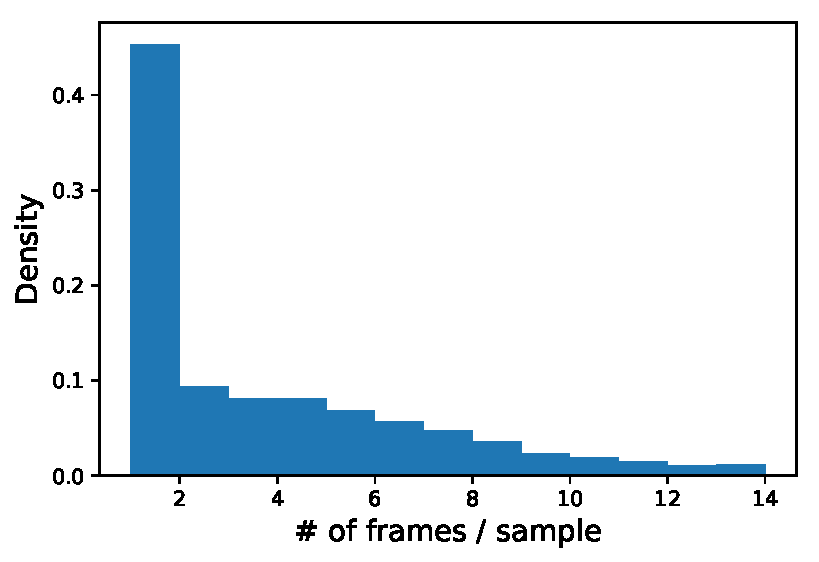
\includegraphics{figures/n_frames_dist.pdf}
    \caption[Distribution of number of frames]{Distribution of number of frames.}
    \label{fig:frames-dist}
\end{figure}

For the proposed model, we can see that it consistently outperforms the two baselines regardless of the configuration.
Also, adding the attention mechanism always improves the accuracy by at least one percentage point. This demonstrates the efficacy of attention mechanisms in the frame tracking task.
Another important point is the effect of shuffling training samples. At first, we train the model without shuffling, i.e. using the same order as they appear in dialogues. However, even with the intrinsic order relation between samples, the training still benefits a lot from shuffling, leading to the best result in Table \ref{tab:baselines}.

%[training time]


\section{Attention mechanisms} \label{sec:att}
\begin{table}
    \centering
    \caption[Accuracy scores of different attention mechanisms]{Accuracy scores of different attention mechanisms.}
    \label{tab:att-res}
    \begin{tabular}[t]{lrr}
        \toprule
        Attention mechanisms & GRU & BERT \\
        \midrule
        No attention & $79.5 \pm 0.65$ & $81.0 \pm 0.73$ \\
        Content-based & $79.6 \pm 1.09$ & $81.9 \pm 0.77$ \\
        Cosine & $80.7 \pm 0.33$ & $81.3 \pm 0.93$ \\
        Dot product & $\bm{82.8 \pm 0.52}$ & $82.3 \pm 1.70$ \\
        Scaled dot product & $81.9 \pm 1.02$ & $\bm{83.0 \pm 0.38}$ \\
        General & $82.4 \pm 0.80$ & $82.4 \pm 0.11$ \\
        Query-key & $82.6 \pm 0.81$ & $82.7 \pm 0.56$ \\
        %Scaled general & $? \pm ?$ & $? \pm ?$ \\
        Scaled query-key & $81.3 \pm 0.55$ & $82.5 \pm 1.70$ \\
        \bottomrule
    \end{tabular}
\end{table}

We further investigate different attention mechanisms. The definition of each mechanism is in Table \ref{tab:att} and the results are shown in Table \ref{tab:att-res}.

First, we notice that all attention mechanisms outperform our no attention baseline model, strengthen our claim about the advantage of attention in frame tracking.
For the comparisons between attention mechanisms, we can see that the accuracy scores of content-based attention are rather low and are even worse than most attention mechanisms. This suggests the importance of having attention scores depending on NLU label embeddings.
On the other hand, there is no clear winner among these attention mechanisms: scaled dot product obtains the best result in the table, but its accuracy is only moderate with LSTM as text embedding.
Nonetheless, the results of dot product, general and query-key are good for both text embeddings.


\section{Hyperparameter tuning}
\begin{table}
    \centering
    \caption[Results of hyperparameter search]{Results of hyperparameter search.}
    \label{tab:hyperopt}
    \begin{tabular}{lrr}
    % {"82.9 ± 1.10", "Attention": "Query-key", "Input dim.": 128, "Hidden dim.": 256, "Embed dim.": 64, "Att. dim.": 64}
    % {"83.0 ± 0.66", "Attention": "Query-key", "Input dim.": 256, "Hidden dim.": 128, "Embed dim.": 64, "Att. dim.": 32}
        \toprule
         & GRU & BERT \\
        \midrule
        Accuracy & $82.9 \pm 1.10$ & $83.1 \pm 0.48$ \\
        \midrule
        Attention & Query-key & Scaled query-key \\
        Input dim. & 128 & 256 \\
        Hidden dim. & 256 & 128 \\
        Embed dim. & 64 & 64 \\
        Attention dim. & 64 & 32 \\
        %What else? & - & - \\
        \bottomrule
    \end{tabular}
\end{table}

In this section, we do a hyperparameter search to see how far we can push the accuracy. We use a Python library called hyperopt \cite{bergstra2013hyperopt}. It searches the hyperparameter space using Tree-structured Parzen Estimator (TPE), which can find good hyperparameters with fewer trials comparing to random or grid search.
% Bergstra, J., Yamins, D., Cox, D. D. (2013) Making a Science of Model Search: Hyperparameter Optimization in Hundreds of Dimensions for Vision Architectures. To appear in Proc. of the 30th International Conference on Machine Learning (ICML 2013).

The hyperparameters we tune include attention mechanisms and dimensions in the model. For the dimensions, we put them into three groups: input, hidden, and embedding. The input dimension is the output dimension of text embedding, slot embedding, and act embedding. The hidden dimension is the dimension of the two GRUs in the NLU label encoder and the frame encoder. The embedding dimension is the output dimension of the two encoders. The options for these dimensions are 64, 128, 256, 512. For attention mechanisms, we consider no attention and all the seven mechanisms in Table \ref{tab:att}. Additionally, there are two query-key attention with different attention dimensions, i.e.\ the output dimension of linear transforms $W_q$ and $W_k$: one is 32 and the other is 64. So there are in total $4^3 \times 9 = 576$ points in this hyperparameter space. The dimension we use in previous results is 128 for input, hidden and embedding dimension, and 64 for the query-key attention dimension.

We do a hyperparameter search for both GRU and BERT text embeddings. The results are in Table \ref{tab:hyperopt}. For both text embeddings, the accuracy scores are improved by $0.1$ percentage point. Besides, the results show that the query-key and scaled query-key attention mechanisms are the best among all attention mechanisms. This is consistent with the observation in Section \ref{sec:att}.

\section{Transfer learning}

\begin{table}
    \centering
    \caption[Accuracy scores with transfer learning]{Accuracy scores with transfer learning. Attention is dot product. The best results in each column are marked bold.\newline}
    \label{tab:transfer}
    \resizebox{\columnwidth}{!}{
        \begin{tabular}{lrrrr}
            \toprule
            Pre-training set & GRU w/o attention & GRU w/ attention & BERT w/o attention & BERT w/ attention \\
            \midrule
            % 0 & $79.1 \pm 0.30$ & $82.3 \pm 0.96$ & $77.5 \pm 0.52$ & $81.0 \pm 0.69$ \\
            % 0 shuffle & $79.5 \pm 0.65$ & $82.8 \pm 0.52$ & $81.0 \pm 0.73$ & $82.3 \pm 1.70$ \\
            Syn. 1 & $77.7 \pm 0.64$ & $81.0 \pm 0.26$ & $79.8 \pm 1.37$ & $82.0 \pm 0.97$ \\
            Syn. 2 & $76.9 \pm 1.21$ & $80.4 \pm 0.64$ & $79.8 \pm 0.75$ & $80.5 \pm 0.91$ \\
            Syn. 3 & $76.9 \pm 0.42$ & $80.0 \pm 0.43$ & $79.7 \pm 1.14$ & $\bm{82.4 \pm 0.42}$ \\
            Syn. 1 + 2 & $78.2 \pm 1.24$ & $\bm{81.4 \pm 0.63}$ & $80.2 \pm 0.53$ & $82.0 \pm 1.80$ \\
            Syn. 1 + 3 & $77.7 \pm 0.73$ & $\bm{81.4 \pm 0.53}$ & $79.8 \pm 0.41$ & $82.3 \pm 0.93$ \\
            Syn. 1 + 2 + 3 & $\bm{78.9 \pm 0.48}$ & $81.1 \pm 0.25$ & $\bm{80.5 \pm 0.52}$ & $82.0 \pm 0.60$ \\
            \bottomrule
        \end{tabular}
    }
\end{table}
In this section, we study how transfer learning can help in frame tracking. We use the large synthetic datasets described in Section \ref{sec:syn} as pre-training datasets and fine-tune the pre-trained model on FRAMES dataset. We use $80\%$ of the pre-training dataset for training and the rest for validation. The model is trained for $20$ epochs and the one having the best validation score is used as the starting point of fine-tuning. The fine-tuning process is the same as in Section \ref{section:setting}.

We experiment with different combinations of synthetic datasets. The description of the datasets is in Table \ref{tab:syn}.
%Among these combinations, there are pretraining sets of different size. In terms of dialogue domain, the third synthetic set is the most relavent to FRAMES dataset. 
The result is in Table \ref{tab:transfer}.
We see again that using attention improves accuracy. As for the comparison between pre-training sets, it is hard to conclude which one is better in terms of accuracy. The best result after fine-tuning is slightly worse than that of training from scratch (cf.\ Table \ref{tab:baselines}).
However, if we look at the learning curves in Figure \ref{fig:curve}, we see that the pre-trained models always start with higher accuracy, showing the advantage of pre-training at the beginning of fine-tuning. Furthermore, they also converge faster. After a few epochs, models training from scratch overtake pre-trained models.

\begin{figure}
    \centering
    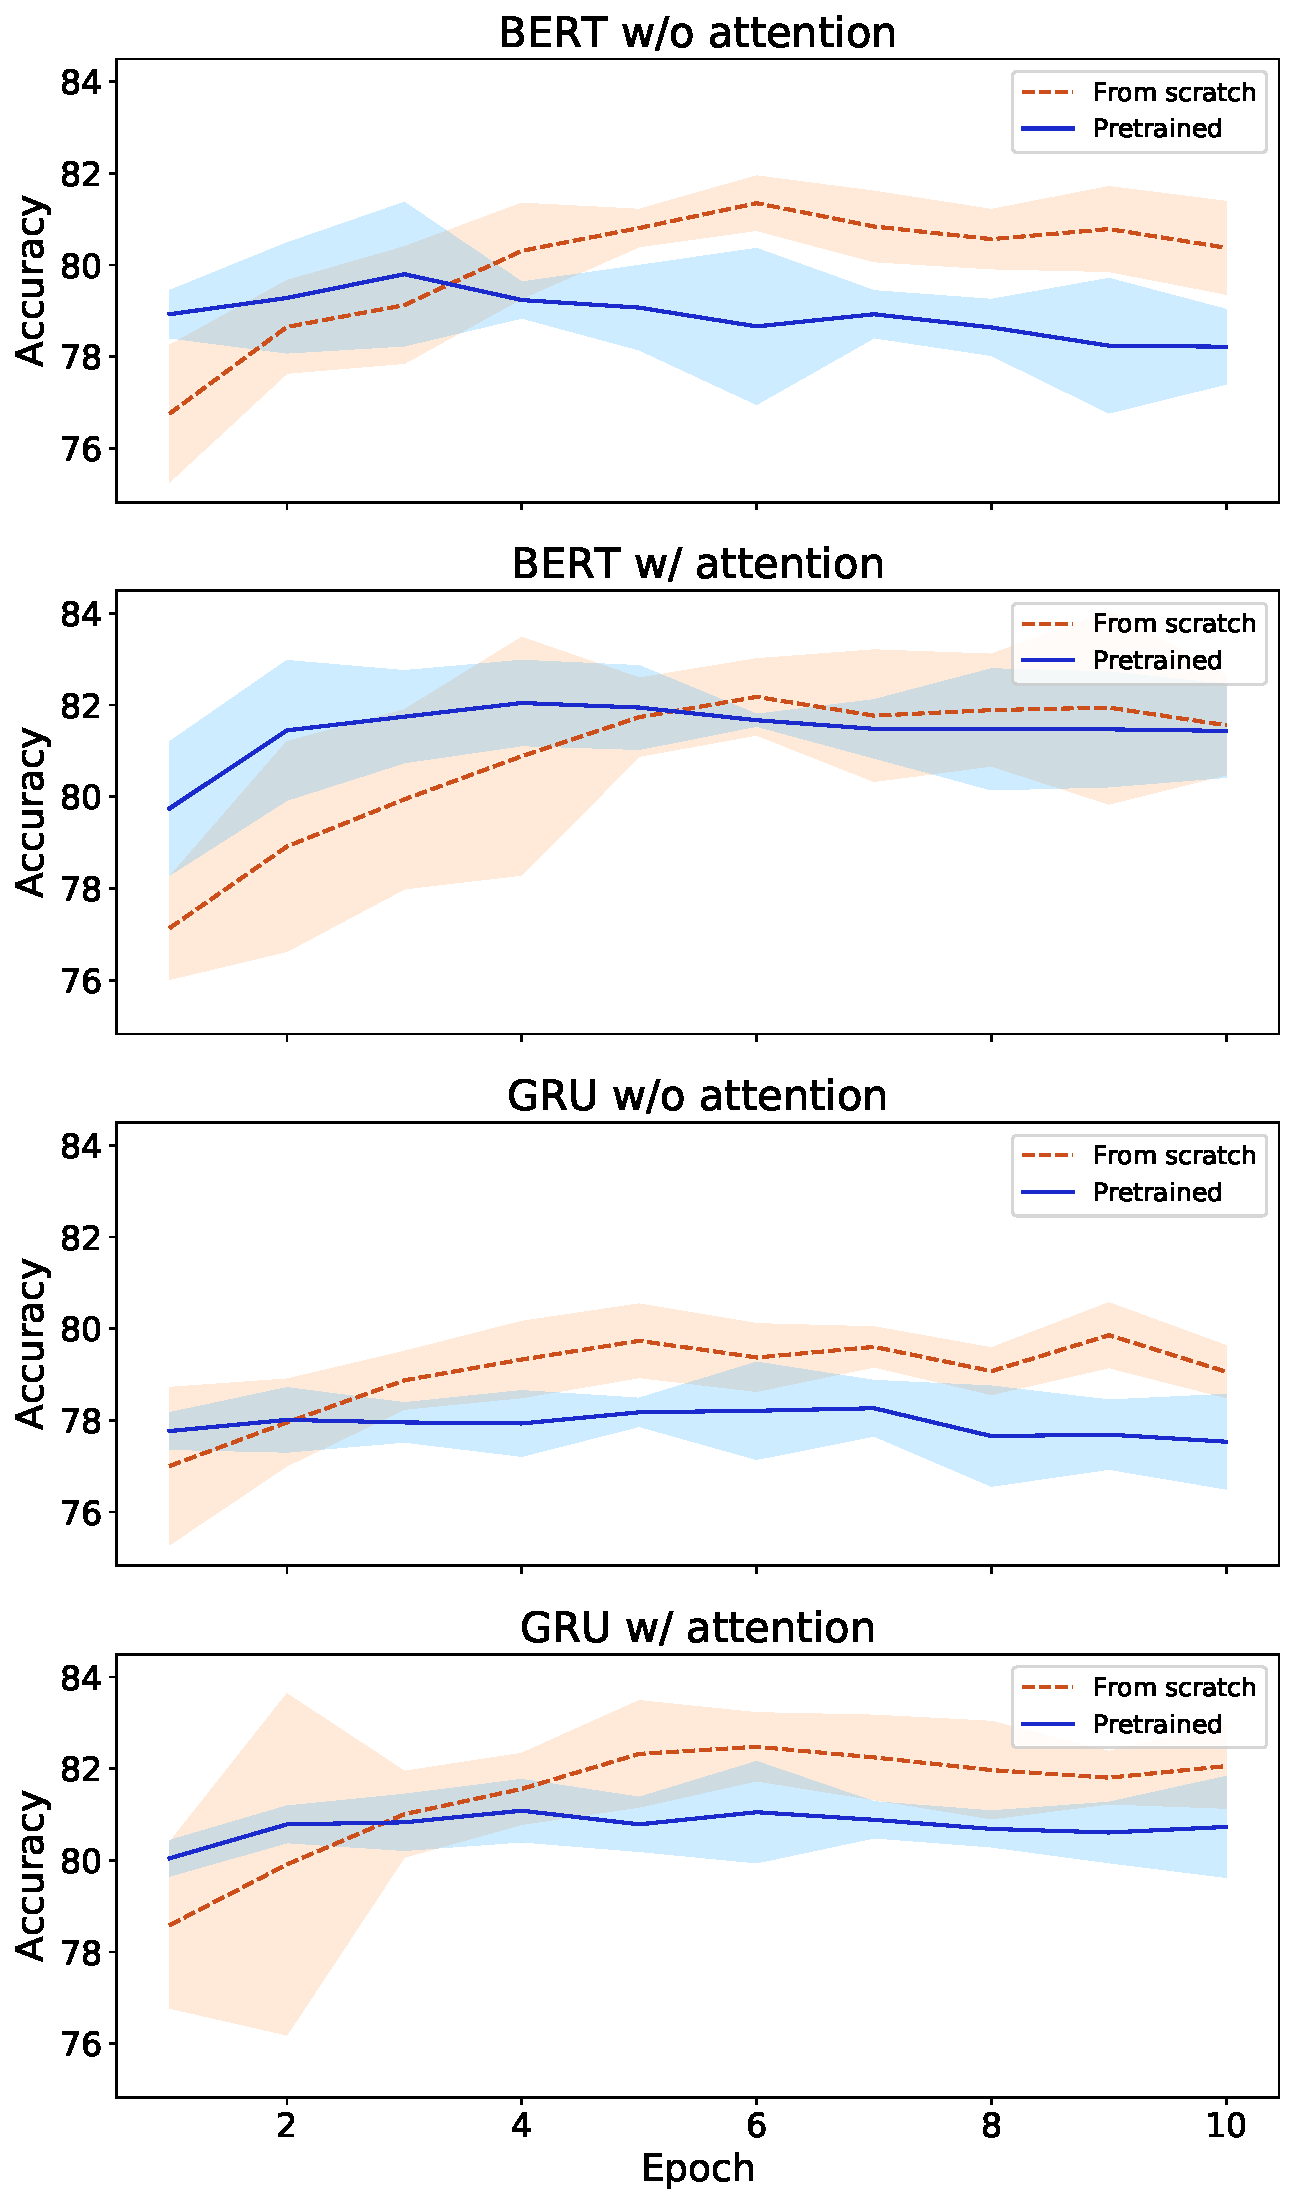
\includegraphics[width=0.8\linewidth]{figures/learning_curves.pdf}
    \caption[Learning curves of transfer learning]{Learning curves of transfer learning. The pre-traning set is synthetic 1.}
    \label{fig:curve}
\end{figure}
